\documentclass[a4paper,11pt]{article}
\usepackage[margin=2cm]{geometry}
\usepackage{multirow}
\usepackage{longtable}
\usepackage[nodayofweek]{datetime}
\usepackage{cite}
\usepackage{graphicx}
\usepackage{url}
\usepackage{tabularx}
\longdate

\usepackage{hyperref}
\usepackage{fancyhdr}
\pagestyle{fancyplain}
\fancyhf{}
\lhead{\fancyplain{}{M.Sc.\ Group Project Report}}
\rhead{\fancyplain{}{\today}}
\cfoot{\fancyplain{}{\thepage}}

\setlength{\parindent}{0em}
\setlength{\parskip}{1em}


\title{Dragonfly Neural Simulation \\\Large{--- Report One ---}}
\author{Alex Carver, Chris Snowden, Desy Kristianti, \\
        Georgios Kontogiannis, Luka Milic, Zoe Landgraf\\
       \{anc15, cps15, dk2015, gk513, lm1015, zl4215\}@ic.ac.uk\\ \\
       \small{Supervisors: Professor Murray Shanahan, Zafeirios Fountas, Pedro Mediano}\\
       \small{Course: CO530, Imperial College London}
}

\begin{document}
\maketitle

\section{Introduction}

\par This project is to develop a neural system that mimics the predatory behaviour of dragonflies, building on previous work \cite{GITHUB1} which has implemented parts of this simulation in a batch process. The particular interest in dragonflies' neural function arises from their efficiency during pursuit, based on selective neural activity. This selection mechanism is driven by the Centrifugal Small Target Motion-Detector Neuron 1 (CSTMD1).

The project's primary focus is to build a module simulating this CSTMD1 with a Hodgkin-Huxley neuron model \cite{Hodgkin} and employ its selection mechanism in a biomimetic agent that exhibits attention-like target selection when performing a simple predation task. The existing modules comprise the functionalities of target detection, pattern recognition and reinforcement learning, as well as a simulation environment. In addition to the central component, the CSTMD1, a Motor Controller will be added, which coordinates the dragonflies' movement in the environment according to pattern recognition of the CSTMD1 output. In order to create a realistic system, the existing and new components will be integrated and adjusted to enable a continuous flow rather than batch execution, a necessity for the model to operate in a real environment. 

\section{Project Structure}

\par We plan to achieve such a mechanism by implementing and bridging the following six components:

\begin{figure}
  \centering
    \makebox[\textwidth]{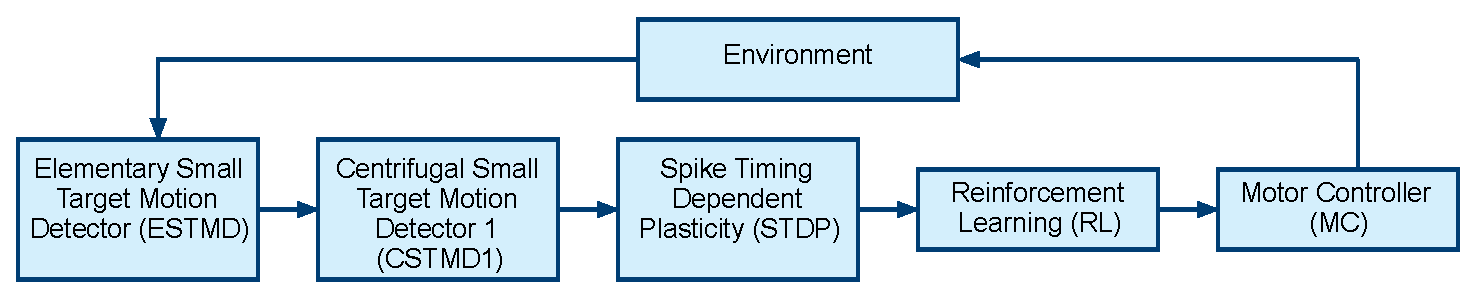
\includegraphics[width=\textwidth]{Project_Structure.eps}}
  \caption{Simulation pipeline}
  \label{modules}
\end{figure}


 \par \textbf{ESTMD}: A series of frames will be passed as input to an \textbf{Elementary Small Target Motion Detector}, which will identify and isolate small moving targets from a noisy background\cite{ESTMD1} and generate neural spikes\cite{ESTMD2}, and then pass the information\cite{ESTMD3} on to the CSTMD1.
 \par \textbf{CSTMD1}: The \textbf{Centrifugal Small Target Motion Detector 1} is the core of the project, implemented as a multicompartmental bistable neuron model\cite{CSTMD1}, which will choose a single target and ignore others. Depending on the input, the neuron will fire a specific repeatable pattern of spikes which will be passed to the STPD. The model will utilise reconstructed morphology based off previous academic research  \cite{Geurten3277}.
 \par \textbf{STDP} The \textbf{Spike Timing Dependent Plasticity} mechanism will learn how to recognise patterns \cite{stdp1}\cite{stdp2} in the output of the CSTMD1 and parse them into distinct signals for the action selection components (RL and MC).
 \par \textbf{RL}: The \textbf{Reinforcement Learning} component use a neural network to associate the recognised patterns \cite{IZ1} it has received with a set of possible actions by the Motor Controller. After the action has been performed, it will then alter the neural network weightings based upon the effectiveness of the action.
\par \textbf{MC}: The \textbf{Motor Controller} will perform an action selected by the RL on the dragonfly's state within the environment.
\par \textbf{Environment}: This will keep track of the position of the predator and will generate moving prey. It will construct frames for the predator's view which will be passed to the ESTMD. Ultimately we aspire to replace this module with a camera mounted drone.
  
\section{Project Goals}

\par Goal-oriented-capture allowed the team to determine the goals and requirements for the project from all stakeholders . These were found to include goals relating to both neurodynamic and computational performance. Figure \ref{goc} is a visual representation of the process the team undertook in order to fully formulate the specification. 

\begin{figure}[b!]
  \centering
    \makebox[\textwidth]{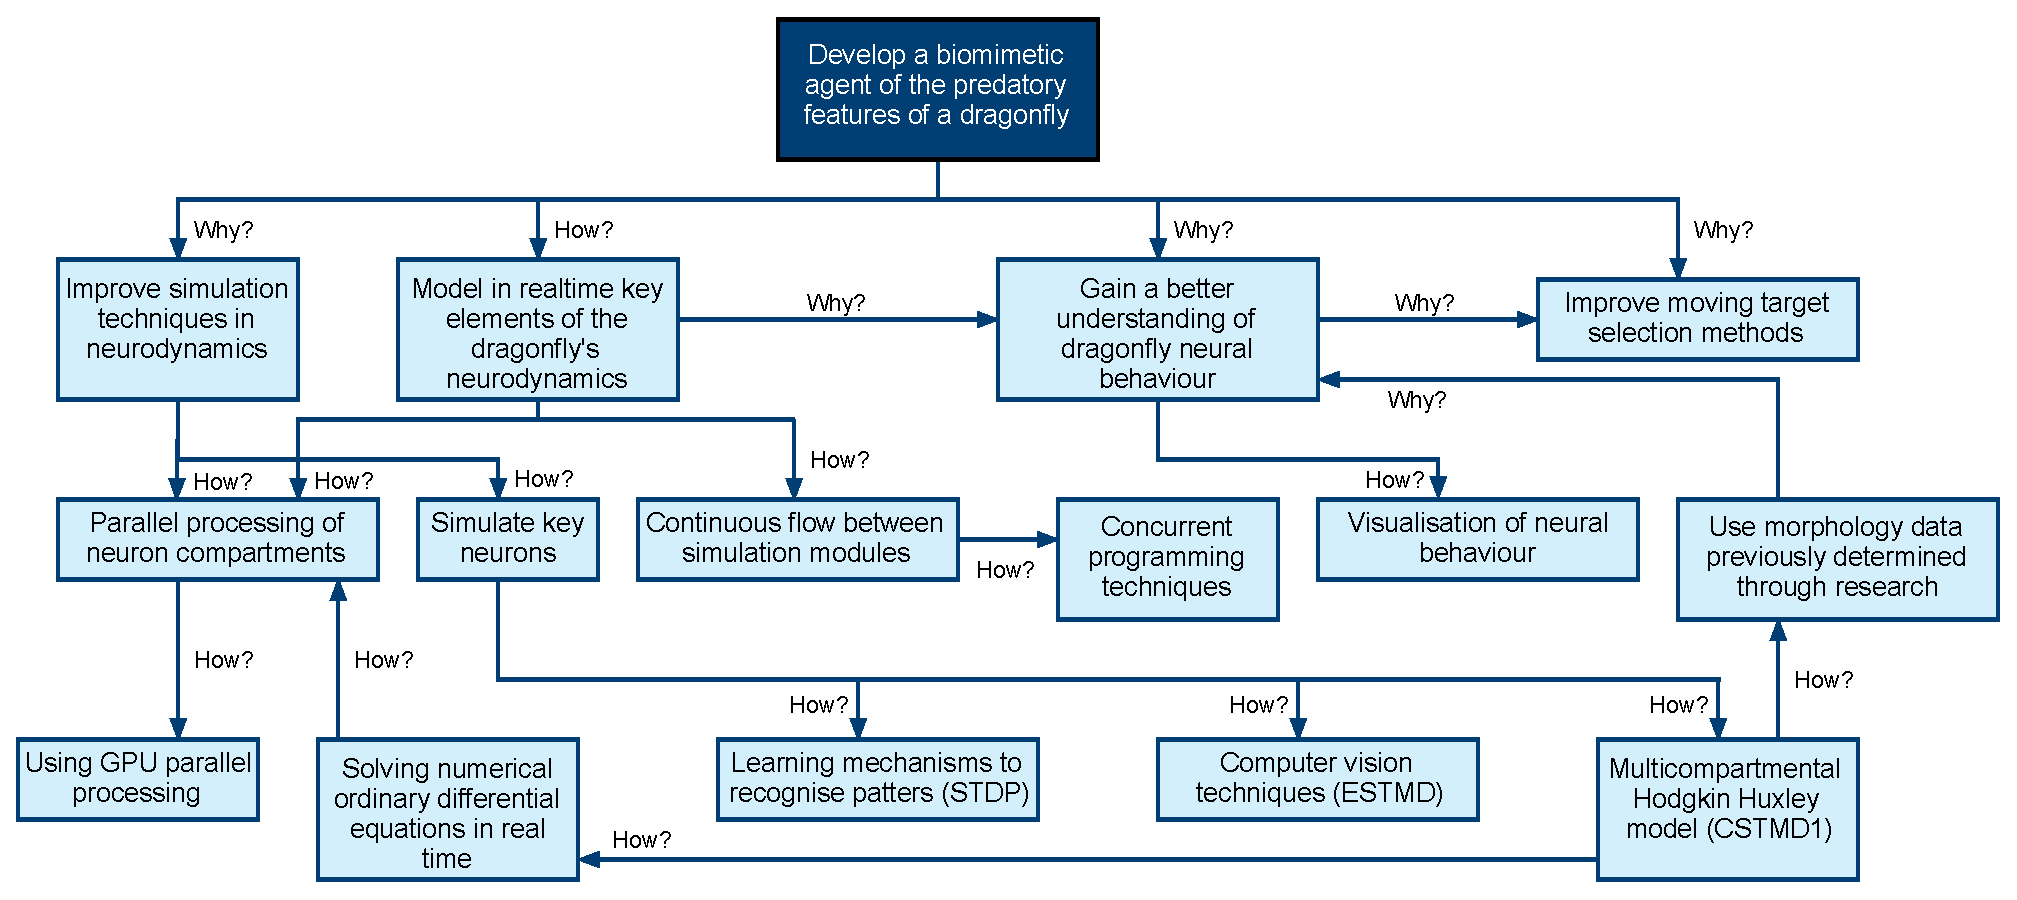
\includegraphics[width=\textwidth]{RequirementsCapture.eps}}
  \caption{Goal-oriented-capture}
  \label{goc}
\end{figure}

\newpage

\par The goal oriented capture coupled with discussions with our supervisors over the extent of existing research allowed us to estimate the level of complexity for each component and split their functionality into three stages of development. The resulting specification is shown in Table \ref{table:req}.

\begin{table}[h!]
\begin{tabularx}{\hsize}{c | c |X}
\multirow{8}{*}{\rotatebox[origin=c]{90}{Minimal}} & A1 & Develop an efficient implementation of a multicompartmental Hodgkin-Huxley neuron model \\
& A2 & Apply this model to create a CSTMD1 simulation \\
& A3 &Integration of ESTMD, STPD and RL with the CSTMD1 neuron(s) into a continuous flow simulation \\
& A4 &2D environment in which the agent will attempt to capture prey \\
& A5 &Implement and integrate a motor module which moves the dragonfly within the environment and automatic system\\
\hline
\multirow{5}{*}{\rotatebox[origin=c]{90}{Full}}
& B1 & Providing a transparent interface in order to understand the characteristics of each module \\
& B2 & Create and display a visualisation of agent's neural behaviour \\
& B3 & The CSTMD1 module exhibiting all theoretically expected features\\
& B4 & Comparison of our own simulation with 3$^{rd}$ party simulators including NEURON \\
& B5 & The connected modules should be able to run in an approximation of real-time\\
\hline
\multirow{5}{*}{\rotatebox[origin=c]{90}{Extensions}}
& C1 & Create a user interface for the virtual simulation environment \\
& C2 & Implement with real-time input from camera \\
& C3 & Extend the enviroment and motor controller to improve realism \\
& C4 &Implement on a simple physical robot or quad-copter \\ 
\end{tabularx}
\caption{Project Specification/Requirements}
\label{table:req}
\end{table}
\section{Development Methodology} \label{developmentMethodology}

 Since our project has complex, interdependent modules that require implementation in different phases, and a large number of possible extensions, we have chosen to utilise an iterative Agile development practice with Scrum methods.

 The project has been split into smaller goals which have been priotised into sprints (see Section \ref{taskscheduling}). We also have decided to apply the practice of pair programming for these sprints. Tasks from a sprint will be assigned to a pair who will work together and review each other's code. At the end of each sprint, one member of the pair shall be cycled to work on a different module. This mitigates the risk last year's group encountered of individual specialisation (see Section \ref{projectrisks}) by ensuring each group member gains experience of each of the modules, whilst simultaneously ensuring a developer with experience of the module is involved with it.

We are currently using Slack, a communication platform for internal project communiation. Each module has a dedicated slack channel allowing for efficient communication between team members working on the same functionality. Task management and assignment will be handled using online task collaboration tool Trello, which will manage the tasks involved for the goals of each sprint. We decided to use Git as our version control system with our remote repository hosted on the Imperial Department of Computing GitLab. 
\section{Task scheduling} \label{taskscheduling}
\par  Seven sprints have been planned for this project, with goals having a priority form 1 (highest) to 3 (lowest). We aim to achieve the core aim of the functioning CSTMD and ESTMD modules linked together by the end of the third sprint, a fully functional and integrated system by the end of the fifth sprint, with the final two sprints dedicated to improvments and exploring potential extensions. We will meet with supervisors Zafeirios Fountas and Pedro Mediano on a weekly basis to review the progress of these sprints as well as plan the next sprint.

\begin{center}
    \begin{tabular}{l p{1.4cm} p{1.4cm} p{1.4cm} p{1.5cm} p{1.4cm} p{1.4cm} p{1.8cm}}
    \textbf{Sprint} & 1 & 2 & 3 & 4 & 5 & 6 & 7(extended) \\
    \hline
    \textbf{Start ('16)}
    &18 Jan & 1 Feb & 15 Feb & 29 Feb & 14 Mar & 28 Mar & 11 Apr \\
    \textbf{End ('16)}
    &31 Jan & 14 Feb & 28 Feb & 13 Mar & 27 Mar & 10 Apr & 1 May\\
    \end{tabular}
\end{center}

\begin{center}
    \begin{longtable}{c | p{12cm} c c}
     \caption{Task prioritisation and scheduling} \\
    &\textbf{Task} & \textbf{Priority} & \textbf{Sprint} \\ \hline
    \endhead
    \parbox[t]{2mm}{\multirow{9}{*}{\rotatebox[origin=c]{90}{CSTMD1}}}
    & Generate CSTMD1 morphology using Python and MATLAB script & 1 & 1 \\
    &Implement multicompartmental Hodgkin Huxley neuron on GPU  & 1 & 1 \\
    &Implement morphology as a GPU neuron model  & 2 & 1 \\
    &Develop 3D visualisation tool & 2 & 1 \\
    &Generate  and implement synapses from individual neuron morphologies  & 1 & 2 \\
    &Integrate ESTMD1 output stimulus & 1 & 3 \\
    &Model verification and parameter search & 1 & 3 \\
    &Re-implement for step simulator for continious flow model  & 2 & 3 \\
    &Integrate with STDP & 1 & 4 \\
    \hline
    \multirow{5}{*}{\rotatebox[origin=c]{90}{ESTMD}}&Analyse and test current ESTMD module for usage and perfomance & 1 & 2 \\
    &Make necessary changes for continuous flow model & 1 & 3\\
    &Integrate with CSTMD1 & 1 & 3 \\
    &Link with Environment & 1 & 3\\
    &Investigate poissible implementation in CUDA and OpenCV & 2 & 4 \\
    \hline
    \parbox[t]{2mm}{\multirow{3}{*}{\rotatebox[origin=c]{90}{STDP}}}
    & Analyse and test current STDP module for usage and performance & 2 & 2 \\
    & Implement into continous flow model & 1 & 4 \\
    & Integrate with CSTMD1 and RL & 2 & 4 \\
    \hline
    \multirow{3}{*}{\rotatebox[origin=c]{90}{RL}}
    & Analyse and test current RL module for usage and performance & 2 & 2 \\
    & Implement into continous flow model & 1 & 4 \\
	& Integrate with CSTMD1 and STDP & 2 & 4 \\
    \hline
	\multirow{3}{*}{\rotatebox[origin=c]{90}{MC}} & Implement motor controller & 1 & 3 \\
	& Integrate with Environment & 2 & 3 \\
	& Integrate with RL & 1 & 4 \\
    \hline
    \multirow{5}{*}{\rotatebox[origin=c]{90}{Environment}}
    &Analyse and test current animation module for usage and performance & 1 & 1 \\
    & Implement 2D environment model including agent and prey location & 1 & 2 \\
    & Extend animation visutalion onto 2D model & 1 & 3 \\
	&Integrate with ESTMD & 2 & 3 \\
	&Build and integrate 3D environment & 2 & 5 \\
    \hline
    \multirow{5}{*}{\rotatebox[origin=c]{90}{Integration}}
    &Integrate current dependencies into a Docker module & 2 & 2 \\
    &Brain Studio investigation for module integration & 2 & 3 \\
    &Investigate Shared memory use for module integration & 2 & 3 \\
    &Testing, quality control and dependency checking & 1 & 5 \\
	&Quad-copter implementation & 3 & 6 \\
	\end{longtable}
\end{center}
\section{Work Allocation}

\par Chris Snowden has been selected to be the leader of the project and is responsible for establishing collaboration methods and coordinating group meetings. Secretarial tasks will be assigned to a different person, rolling weekly, with overall supervision by Zoe Landgraf. Group members will be cycled between these modules as described in Section \ref{developmentMethodology}, to ensure all group members gain experience in working and understand the code for all modules. For the current sprint (2) the pairs are: Alex Carver and Georgios Kontogiannis (ESTMD), Chris Snowden and Luka Milic (CSTMD1) and Desy Kristianti and Zoe Landgraf (Environment, STDP, RL and Integration).

\iffalse

\par The table below shows the initial focus allocated work so far:

\begin{table}[ht]

\centering % used for centering table

\begin{tabular}{l c c c c c c} 
 & Environment & ESTMD & CSTMD1 & STDP & RL & MC\\ [0.5ex]

\hline 

Alex Carver & & x & & & x & x  \\ % inserting body of the table

Christopher Snowden & & & x & & & x  \\

Desy Kristianti & x & & & x & & x  \\

Georgios Kontogiannis & & x & & & x & x \\

Luka Milic & & & x & & & x \\

Zoe Landgraf & & & x & x & & x \\ [1ex] % [1ex] adds vertical space

\end{tabular}

\label{table:nonlin} % is used to refer this table in the text

\end{table}

\fi
\section{Project Risks} \label{projectrisks}

\par  There may be significant overhead required for the team to become fully acquainted with the neurodynamic concepts needed. As such we are maintaining open channels of communication with our supervisors and have completed background reading following an initial project meeting on 16$^{th}$ December 2016.

\par Associated with this overhead is the need (see requirement B3), not only to produce functioning code, but also a model that exhibits the same characteristics as those found in published experiments. In order to mitigate this we are developing the CSTMD1 iteratively and at a high priority to ensure that it is accurate so other modules can be developed from it. A visualiser has also been developed allowing the team to observe the voltage changes through the dendritic tree.

\par Because of the complexity of each module, it will be advantegous to have a group member with experience of a module working on it at all times. However, last year's group encountered the problem of excessive independant specialisation\cite{GITHUB2}, and when problems arose with a specific module other group members were too inexperienced with the module to aid in its development. To mitigate this risk whilst also retaining experience, group members will alternatively cycle between modules every two sprints, keeping an experienced developer on a module whilst ensuring all members gain experience over all modules.

\iffalse
\par Due to project aim to create a pseudo-realtime system there is an ongoing risk that one or more modules cannot operate at the required sample time. Given the feedback from the previous MSc project \cite{GITHUB2} it was seen that the CSTMD1 simulation acted as a bottleneck resulting in an end product that required manual batch data manipulation. During initial work optimisations have already been found in order to minimise the risk associated with computation time including but not limited to removing inefficiecies in the inter-module interactions.
\fi
\section{Project Boundaries}
\iffalse
\subsection{Stakeholders} \label{stakeholders}
\par The project has a strong academic motivation based on academic research currently being undertaken in the Neurodynamics community and within Prof. Murray Shanahan's group. The ultimate goal of the project is to publish a paper in collaboration with both PhD students Pedro Mediano and Zafeirios Fountas and thus make the project's findings available to the wider academic community.
\fi

\iffalse \subsection{Software and Hardware} \fi
The target operating system for the software will be Ubuntu 14.04 as it has long term support from its developers and is a popular stable platform for all the software which we shall use.

Python has many libraries optimised for scientific computing (such as numpy, scipy and matplotlib), and was also used extensively by the group working on this project last year, so will be the language of choice. The exceptions are the CSTMD1 and possibly the ESTMD modules where we will take advantage of GPUs with the CUDA platform combined with the Thrust and the CUBLAS libraries.

The structure of the project is highly modular hence an integration system will be required.  We will either use Brain Studio, which is in early development by the Computational Neurodynamics group, or exploit the low level features of the operating system to achieve inter-process synchronisation.

For visualisation matplotlib will be used as it is very simple and lightweight. For more complex visualisations requiring 3D graphics PyQTGraph will be used. In addition some use of Matlab will be required, particularly for generating the morphologies of the CSTMD1 neuron.

\iffalse % COMMENT OUT: START
\par Hardware/OS:
\begin{itemize}
  \item Linux / DGB
  \item NVIDIA GeForce
  \item Local / not distributed \ldots
\end{itemize}
\par Dependencies:
\begin{itemize}
  \item CUDA
  \item Numpy
  \item OpenGL
  \item OpenCV
  \item (PyQT)
  \item cuBLAS
  \item Thrust
  \item Gizeh
  \item Brain Studio
  \item Quadcopter
\end{itemize}
\fi % COMMENT OUT: END

\bibliographystyle{unsrt}
\bibliography{report1}
\end{document}

